\subsection*{Short Introduction}
Flow categories originally emerged as a categorical bookkeeping mechanism to organize the geometric and analytic data extracted from Hamiltonian systems on a manifold \cite{CJS95}. In recent years, flow categories and their stable homotopy types have become central tools for lifting invariants in Floer, contact, and Khovanov homology into the realm of stable homotopy theory. A natural question arises: how can we systematically compute the generalized homology of these realization spectra directly from the underlying geometric flow data?   

Here is an intuitive description of the main theorem of the paper using a toy model coming from Morse theory.
Let $\Man$ be a closed manifold and $f: \Man \to \bbR$ a Smale Morse function. Denote by $\mathrm{Crit}(f)$ the set of critical points of $f$, and by $\ind: \mathrm{Crit}(f) \to \bbZ$ the index function. For simplicity, assume that there is one critical point for each index $i \in \{0, \dots, n\}$, and denote the critical points by $x_i$ where $\ind(x_i) = i$.
The first result is:

There is a spectral sequence 
\begin{equation*}
    \pg{E}{1}{n}{p} = \Omega^{\fr}_{n-p} \implies \pi_n \Sinf \Man.
\end{equation*}
where $\Omega^{\fr}_*$ is the framed bordism ring, and $\Sinf \Man$ is the stable homotopy type of  $\Man$.

Let $x_j,x_i$ be two critical points of $f$ with $j > i$. We denote by $\flowM(x_j,x_i)$ the compactification of the moduli space of flow lines from $x_j$ to $x_i$, up to reparametrization. Recall that $\flowM(x_j,x_i)$ is a framed manifold with corners of dimension $\ind(x_j) - \ind(x_i) - 1$, and that the boundary structure is given by
\begin{equation*}
    \partial \flowM(x_j,x_i) = \bigcup_{j > r > i} \flowM(x_j,x_r) \times \flowM(x_r,x_i).
\end{equation*}

Let $W_p$ be a representative of a bordism class in $\pg{E}{1}{n}{p} = \Omega^{\fr}_{n-p}$.
We have that $W_p$ survives to the $(r+1)$-th page (also denoted by $W_p \in Z_{r+1}$) if and only if there is a family of framed manifolds $\{W_s\}$ for $s \in \{p-1, \dots, p-r\}$ of dimension $n-s$ such that the corner structure is given by
\begin{equation*}
    \partial W_s = \bigcup_{p \geq t > s} W_t \times \flowM(x_t,x_s).
\end{equation*}

We can then glue the collection $W_s \times \flowM(x_s,x_{p-(r+1)})$ together.
Let $t,u \in \bbZ$ be such that $p \geq t > u \geq p-(r+1)$. By the definition of the boundary structure of $W_u$ and $\flowM(x_t,x_{p-(r+1)})$, we have that 
\begin{equation*}
    W_t \times \flowM(x_t,x_{p-(r+1)}) \hookleftarrow W_t \times \flowM(x_t,x_u) \times \flowM(x_u,x_{p-(r+1)}) \hookrightarrow W_u \times \flowM(x_u,x_{p-(r+1)})
\end{equation*}
and these boundary components are shared only by these two manifolds of the collection $W_s \times \flowM(x_s,x_{p-(r+1)})$.
On the other hand, all the boundary components of $W_s \times \flowM(x_s,x_{p-(r+1)})$ are of this form, so we can glue the collection $W_s \times \flowM(x_s,x_{p-(r+1)})$ together to obtain a framed closed manifold which we denote by
\begin{equation*}
    \flowM(-,x_{p-(r+1)}) \circ W \coloneqq \bigcup_{s \in \{p,\dots, p-r\}} \flowM(x_s,x_{p-(r+1)}) \times W_s,
\end{equation*}
which is an analog of the Toda bracket construction. Note that 
\begin{equation*}
    \dim(\flowM(x_s,x_{p-(r+1)}) \circ W) = \dim(W_s) + \dim(\flowM(x_s,x_{p-(r+1)})) = n-s + \big(s - (p-(r+1)) - 1 \big) = n-p+r.
\end{equation*}
The last part of the theorem states that if $W_p \in \pg{E}{1}{n}{p} = \Omega^{\fr}_{n-p}$ survives to $Z_{r+1}$, then the $r+!$ differential on $Z_{r+1}$ is given by the bordism class of the Toda manifold: 
\begin{equation*}
    d_{r+1}(W_p) = [\flowM(-,x_{p-(r+1)})\circ W] \in \Omega^{\fr}_{n-p+r} = \pg{E}{1}{n-1}{p-(r+1)}.
\end{equation*}
See \cref{fig:ffCat} for an example of the structure of the family $W_s$ and the flow manifolds,
\cref{fig:k-boundary} for the gluing diagram of the Toda manifold, and \cref{fig:differential} for the resulting closed manifold.


\subsection*{Background}
\textbf{Morse theory basics}. The field of differential topology studies the connection between analysis on a smooth $n$-manifold $M$ and its underlying topology. This field was pioneered by Morse in the beginning of the 20th century, and further developed by Smale, Thom, Milnor and more (see \cite{morse1925relations} for Morse first work and \cite{milnor1963morse} for Milnor’s classic exposition of the subject).
To begin understanding $\Man$, we take a ``nice'' (namely a Smale-Morse) function $f \colon \Man \to \bbR$. We extract the \emph{critical points} of $f$ and, for any critical point $p$, assign its \emph{index} $\ind(p)$ - which is defined as the signature of the Hessian of $-\nabla f$. Pictorially, this index represents the number of ‘downward’ axes at $p$, see \cref{fig:Heart}.

For any two critical points $y$ and $x$, we define $\nonflowM(y, x)$ to be the moduli space of curves (up to reparametrization) in $\Man$ that start at $y$ and end at $x$, and follow the gradient field $-\nabla f$. We call such curves \emph{flow lines}; see \cref{fig:Heart}. Under generic conditions, $\nonflowM(y, x)$ is a smooth (not necessarily closed) manifold of dimension $ \ind(y) - \ind(x) - 1 $.

\textbf{Framed flow manifolds}. Our main interests are \emph{flow manifolds}, which are the compactification
\begin{equation*}
    \flowM(y,x) \coloneqq \overline{\nonflowM(y,x)}.
\end{equation*}

\begin{figure}[h]
\centering
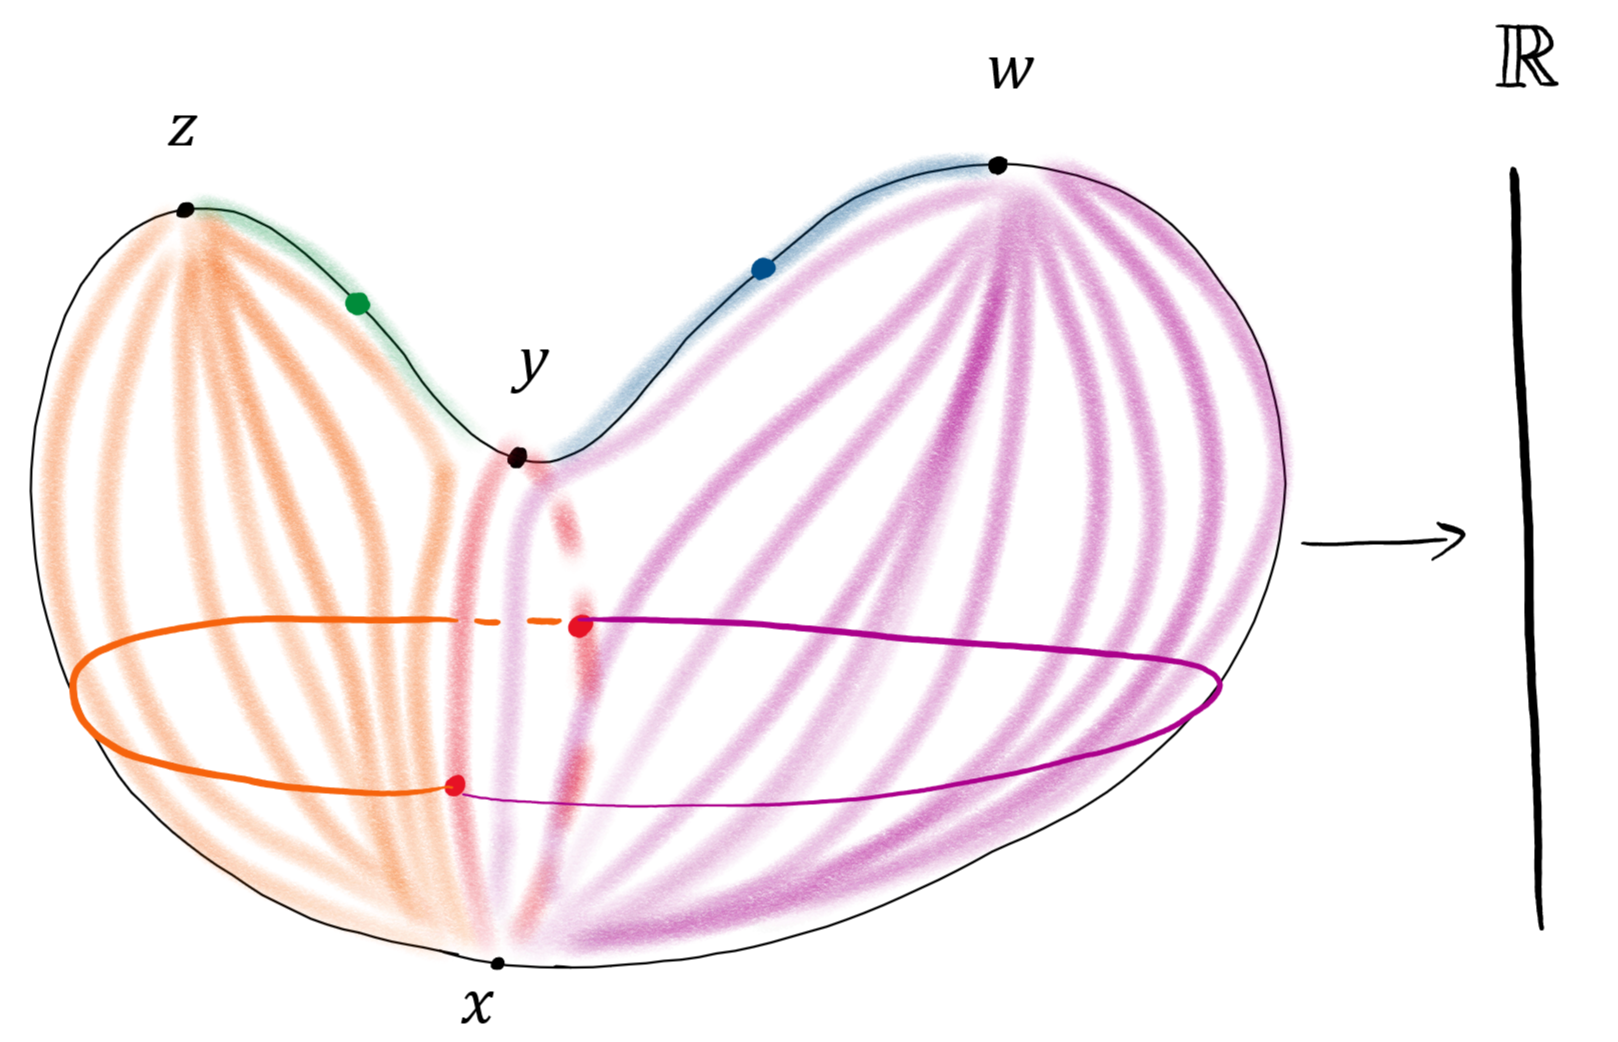
\includegraphics[scale=0.33]{fig/Heart.png}
\caption{A Smale-Morse function on the sphere, given as projection to the $z$ axis of the heart-shaped embedding. The letters represent critical points (with indices 2,2,1,0), the flow lines are drawn as soft, colorful lines, the solid colorful dots are representatives for the zero-dimensional flow manifolds and the solid colorful lines are representatives for the one-dimensional flow manifolds (notice the boundary structure as broken flow lines)}\label{fig:Heart}
\end{figure}

The compactification is given by adding \emph{broken flow lines}, which are piecewise smooth curves that start at $y$ and end at $x$ and pass through other critical points. We get that the flow manifolds have a \emph{corner structure}
\begin{equation*}
    \partial \flowM(z,x) = \bigcup_{\ind(z) > \ind(y) > \ind(x)} \flowM(z,y) \times \flowM(y,x).
\end{equation*}

see \cref{fig:Heart}. The fact that $\flowM(y,x)$ is constructed form the transverse intersection of two discs (one for curves ascending to $y$ and one for curves descending to $x$) gives a stable \emph{framing} on $\flowM(y,x)$ - a trivialization of the form 
\begin{equation*}
    T\flowM(y,x) \oplus \underline{\bbR}^{\ell_1} \overset{}{\simeq} \underline{\bbR}^{\ell_2}
\end{equation*}
where $\underline{\bbR}^{\ell_i}$ are trivial vector bundles over $\flowM(y,x)$. Moreover, the framing of all the flow manifolds is compatible with the corners structure.

\textbf{Morse homology}. It's worth saying that this data is sufficient to calculate the homology $H_*(M,\bbZ)$. It is given as the homology of the Morse chain complex $(C_*, d)$. The generators of $C_p$ are critical points with index $p$. Given two critical points $y,x$ with $\ind(y) -1 = \ind(x)$, the flow manifold $\flowM(y,x)$ is in fact compact; the coefficient of $x$ in $d(y)$ is given by the signed count of $\flowM(y,x)$, where the signs are determined by the framing. The boundary structure of the one-dimensional moduli spaces $\flowM(z, x)$ shows that $d^2 = 0$. See \cite{schwarz1993morse}.

\textbf{Bordism and generalized homology}. The fact that the flow manifolds are framed hints at an important theorem in differential topology, the Pontryagin-Thom isomorphism. We say that two closed framed $n$-manifolds $M_1$ and $M_2$ are \emph{bordant} if there is a framed $(n+1)$-manifold $W$, with $\partial W = M_1 \sqcup M_2$, in a way that is compatible with the framing. We denote by $\Omega^{\fr}_n$ the set of $n$ dimensional framed manifolds up to bordism. In fact the collection $\Omega_*^{\fr}$ form a graded ring, by disjoint union and Cartesian product.

The \emph{Pontryagin-Thom isomorphism} states that there is an isomorphism
\begin{equation*}
    \Omega_n^{\fr} \simeq \colim_k [S^{n+k},S^k]
\end{equation*}
between bordism groups of framed manifolds and stable homotopy groups of spheres (see \cite{pontryagin1955smooth, thom1954quelques}). The right hand side is also known as the coefficient ring $\pi_n(\bbS)$, where $\bbS$ is the spectrum representing stable homotopy.
We can view the Morse chain complex as a chain complex with coefficient ring $\bbZ = \Omega_0^{\fr} = \bbS_{\leq 0}$ and the differential is given by multiplication by the 0 dimensional flow manifolds $\flowM(y,x)$.

\textbf{Floer theory} A related question is the analysis of real-valued functions on objects that are not finite-dimensional closed manifolds. Floer developed this idea in the 1980s, leading to what is now known as Floer theory.
In general, Floer's idea is to generate a chain complex in which the differentials are defined by 'counting solutions' to a moduli problem (see \cite{floer1987morse} for initial formulations of this idea). In this case, the outcome does not yield the homology of a manifold, and one may ask: \textit{Are Floer homology groups merely the shadow of a more structured object?}

\textbf{Flow categories}. The development of a framework to address these questions led Cohen, Jones, and Segal (CJS) in \cite{CJS95} to introduce \emph{framed flow categories}, which axiomatize the data extracted from a Smale-Morse function on a manifold. In short, a framed flow category $\fC$ consists of a set of objects (corresponding to critical points) with a grading function $\norm{-}$ (corresponding to the index). For two objects $y,x \in \fC$, the morphism space from $y$ to $x$ is an ($\norm{y}-\norm{x}-1)$-dimensional manifold with corners, denoted $\flowM_{y,x}$, equipped with a choice of trivialization of $T\flowM_{y,x} \oplus \underline{\bbR^k}$ for some $k$ (corresponding to the stable framing).
Moreover, the composition is given by identifying the faces in the following way:
\begin{equation*}
    \flowM_{z,y} \times \flowM_{y,x} \hookrightarrow \flowM_{z,x}.
\end{equation*}
See \cref{sec:FFCat} for definitions and details.

Another building block in the theory are \emph{flow modules}. Given a flow category $\fC$, a right flow module $W$ over $\fC$ consists of a collection of manifolds $\{W_x\}_{x\in \fC}$, together with corner structure maps \begin{equation*}
    W_y \times \flowM_{y,x} \hookrightarrow W_x.
\end{equation*}
A right flow module is of \emph{degree} $i$ if 
\begin{equation*}
    \dim W_x = i - \norm{x}
\end{equation*}
for each pair of objects $y$ and $x$ in $\fC$. See \cite{porcelli2024bordism} definition 4.6, 4.7.
By abuse of notation, we denote the collection of right modules of degree $i$ over $\fC$ 
\begin{equation*}
    [*[i],\fC].
\end{equation*}
Similarly, we can define left flow modules of degree $i$ to be collections of manifolds $\{V_x\}_{x \in \fC}$, together with corner structure maps
\begin{equation*}
    \flowM_{y,x} \times V_x \hookrightarrow V_y.
\end{equation*}
such that $\dim V_x = \norm{x} - i$. We denote the collection of left modules of degree $i$ over $\fC$ by 
\begin{equation*}
    [\fC, *[i]].
\end{equation*}
A useful example for left module on a category $\fC$ is given by fixing $x' \in \fC$ and taking the collection
\begin{equation}
    \{\flowM_{x,x'}\}_{x \in \fC}.
\end{equation}
Indeed we have that the corner structure is given by the maps
\begin{equation*}
    \flowM_{y,x} \times \flowM_{x,x'} \hookrightarrow \flowM_{y,x'} 
\end{equation*}
The degree of this module is given by
\begin{equation*}
    \norm{x} - \dim (V_x) = \norm{x} - (\norm{x} - \norm{x'} - 1) = \norm{x'} + 1
\end{equation*}
and we denote is just by $\flowM_{-,x'}$.


\textbf{Filtrations and coherent chain complexes}. Another result of CJS was to attach a stable homotopy type to a framed flow category by the following idea.

Given a filtered space $X_0 \to X_1 \to \dots \to X_n = X$ we can take the successive cofibers to produce a ``chain complex" defined by
\begin{equation*}
    K_* \coloneq X_n/X_{n-1} \xrightarrow{d} \Sigma (X_{n-1}/X_{n-2}) \xrightarrow{d} \dots \xrightarrow{d} \Sigma^{n} X_0,
\end{equation*}
where $d^2$ is null-homotopic via the canonical null homotopy arising from $X$. Moreover, viewing $K_*$ from higher-categorical perspective allows us to encode additional data. In particular, there exist two null homotopies for $d^3$ that can be concatenated to form a loop in a suitable mapping space; the chain complex is then equipped with a null homotopy of this loop, and so forth. We call this structure a \emph{coherent chain complex}.
We can attempt to recover $X$ by taking \emph{iterated cofibers}. For example, note that
\begin{equation*}
    \S^2 X_1 = \cof \left (\S^1 X_1/X_0 \to \S^2 X_0 \right ), \quad \S^2 X_2 = \cof \left (\cof (X_2 / X_1 \to \S X_1/X_0) \to \S^2 X_0 \right )
\end{equation*}
and indeed, we can recover $X$ up to a certain suspension. See \cref{subsec:Ch&fil} and \cite{Ari21} for full detailed text.

Building on this idea, CJS showed that a framed flow category $\fC$ can be collapsed,via a Pontryagin-Thom-type construction, into a coherent chain complex $K$ in Spectra. After taking iterated cofiber, we obtain a spectrum
\[
    \norm{\fC} \coloneq \lim_p \cof (\cof (\dots \cof (\cof (K_p \to K_{p-1}) \to K_{p-2}) \to \dots \to K_1) \to  K_0)
\]
which is called the \emph{realization}\labeltext{realization}{txt:real} of $\fC$.
\begin{rem*}
    Note that $\norm{\fC}$ depends on the choice of framing for the manifolds $M_{b,a}$.
\end{rem*}

\textbf{Example - Morse flow category}. To combine the ideas of framed flow categories and chain complexes, let $f: \Man \to \bbR$ be a manifold equipped with a Smale-Morse function. First, we construct from $f$ a framed flow category $\fC_f$ - by taking $\flowM_{y,x} \coloneq \flowM(y,x)$, then we collapse it to a chain complex $K_{\fC_f}$ and realize it as $\norm{\fC_f} \in \Sp$. A result by CJS \cite{CJS95}, states that this procedure recovers the stable homotopy type of $M$:
\begin{equation*}
    \norm{\fC_f} \simeq \Sinf \Man.
\end{equation*}

This framework has proven useful in Floer theory, where the solutions to the moduli problem sometimes exhibit the structure of a flow category $\fC$. In such cases, we can realize the flow category, demonstrating that Floer homology is indeed a shadow of $\norm{\fC}$.

Looking back to Morse homology, we observe that the homology of a flow category can be determined from its zero-dimensional morphism manifolds. The fact that we can recover the stable homotopy type of $\Man$ from its framed flow category motivates the idea that we can read off the (generalized) homology of $\Man$ using the flow manifolds.

This idea goes back to Floer, who pointed out in \cite{floer1989witten} that: If $h_*$ is a general homology theory, trajectory space analysis suggests contributions from compact components of $\flowM(x, y)$. For stable homotopy $h_* = \pi^{s}_*$, this corresponds to the framed cobordism type. While higher-dimensional components of $\flowM(x, y)$ may not be compact, a modified approach could yield a spectral sequence. This framework has limited use in finite-dimensional Morse theory but may apply to infinite-dimensional settings. 


\todo{remove this "intuitive conclusion of introduction"?}\textbf{Gluing it together.} \emph{In this paper, given a flow category, we use the framework of CJS, Lurie, and Ariotta-Krause to generalize Floer’s idea and construct an Atiyah-Hirzebruch-like spectral sequence. This spectral sequence is given explicitly by gluing the flow manifolds.}

One can think of this result as the generalization of Morse and Floer homology in the sense that we provide a recipe for starting with a manifold or Floer data and reading off its generalized homology groups using the geometric and analytic data.

\subsection*{Notations}
We denote by $\Top$ the $1$-category of topological spaces, by $\Spaces$ the category of homotopy types (or $\infty$-groupoids), and $\Sp$ is the category of spectra. The stabilization functor is denoted $\Sinf: \Spaces \to \Sp$, and $\Ch(\Sp)$ and $\Fil(\Sp)$ denote the categories of coherent chain complexes in Spectra and (complete) filtered Spectra, respectively.

For a topological space $Y$, we denote by $Y_+$ its one-point compactification (if $Y$ is compact, then $Y_+ = Y \cup \{*\}$).
For a CW complex $Y$, we denote by $\sk_n Y$ its $n$-th skeleton.

For a stable tangential structure $\xi: \cX \to BO$, we denote by $\Omega^{\cX}_*$ the graded $\cX$-bordism ring and by $M\cX$ the Thom spectrum associated with the $\cX$-structure (see \cref{sec:tangStr} for definitions).

In this paper, a manifold is assumed to be a \emph{closed manifold} unless stated otherwise.

Let $\fC$ be a flow category. For $q,p \in \bbZ$ we denote by $\fC_{[q,p]}$ the full subcategory of $\fC$ consisting of objects satisfying $q \ge \norm{x}\ge p$, and we define $\fC_p \coloneqq \fC_{[p,p]}$. For brevity, we write 
\begin{equation*}
    M_{p,q}\coloneqq \bigsqcup_{y \in \fC_q, x \in \fC_p} M_{y,x}.
\end{equation*}
for the union of the flow manifolds, and for a right / left module over $\fC$ we write
\begin{equation*}
    W_p \coloneqq \bigsqcup_{x \in \fC_p} W_x, \quad V_p \coloneqq \bigsqcup_{x \in \fC_p} V_x.
\end{equation*}

Moreover, for a stable tangential structure $\xi: \cX \to BO$, one can define $\cX$ flow categories as those flow categories in which the morphism manifolds are equipped with an $\cX$ structure that is compatible with composition (in place of a stable framing). For an $\cX$ flow category $\fC$, we obtain a coherent chain complex $K_{\fC} \in \Ch(\Mod_{M\cX})$, and, analogously to the realization in $\Sp$ (see \ref{txt:real}), we define $\norm{\fC} \in \Mod_{\cX}$ to be its iterated cofiber.

\subsection*{Our results}
\label{def:Xrnp-extension}\todo{add begin defn?}
Let $\cX$ be a stable tangential structure, let $\fC$ be a $\cX$-structured flow category.
Let $n,p,r \in \bbZ$ and let $W,V$ be a right and left flow module over $\fC$ of degree $n$ and $p-r$ respectively. We define the punctured cube diagram
\begin{equation*}
    D: \ P(\{p,\dots,p-r\}) \setminus \{\varnothing\} \to \Top,
\end{equation*}
where $P(-)$ denote the power set, by setting
\begin{equation*}
    D(\{a_k, \dots, a_1\}) = W_{a_k} \times \flowM_{a_k,a_{k-1}} \times \flowM_{a_{k-1},a_{k-2}} \dots \times \flowM_{a_2,a_1} \times V_{a_1},
\end{equation*}
where $a_k > a_{k-1} > \dots > a_1$.
The \textbf{Toda manifold} is the colimit which we denote
\begin{equation*}
    V \circ W \coloneqq \colim D 
\end{equation*}
and we will see later that the Toda manifolds indeed have a manifold structure, and that they are closed, $(n-p+r)$-dimensional, $\cX$-structured.

For the spectral sequence, we consider a family of such constructions indexed by objects in $\fC_{p-(r+1)}$. Specifically, for each $z \in \fC_{p-(r+1)}$, we define a punctured cube diagram $D_z$ by replacing the left module $V$ with $\flowM_{-,z}$ in the general construction. This yields a Toda manifold
\begin{equation*}
    \flowM_{-,z} \circ W := \colim D_z \in \Omega^{\cX}_{n-p+r}.
\end{equation*}
Taking the disjoint union over all $z \in \fC_{p-(r+1)}$, we obtain an element
\begin{equation*}
    \bigsqcup_{z \in \fC_{p-(r+1)}} (\flowM_{-,z} \circ W) \in \bigoplus_{z \in \fC_{p-(r+1)}} \Omega^{\cX}_{n-p+r}.
\end{equation*}

\begin{exmp*}
    In \cref{fig:ffCat}, \ref{fig:k-boundary}, and \ref{fig:differential}, we can see an example of an extension and its Toda manifold.
\end{exmp*}

\begin{figure}[h!]
\[
\input{fig/rightLeftBimod Alt.tex}
\]
\caption{
The solid part represents the flow category $\fC$. Its objects are the $x_i$'s with $\norm{x_i}=i$, and the arrows represent the morphism manifolds.
The 0 dimensional framed manifold $w_4$ represents an element in $E_1^{4,4} = \Omega^{\fr}_{4-4}$.
The dashed arrows represent an right module over $\fC_{[4,2]}$.
The symbols $\pm$, $I$, etc., represent the flow manifolds themselves (where $\pm$ represents a framed point; the rest of framing is omitted for clarity).
}\label{fig:ffCat}
\end{figure}

\captionsetup{font={small}}
\begin{figure}[h!]
\centering
\begin{minipage}{.61\textwidth}
  \centering
  \adjustbox{width=\linewidth}{\begin{tikzcd}
{W_4\times M_{4,3}\times M_{3,2}\times M_{2,1}} && |[myyellow]|{W_4\times M_{4,3}\times M_{3,1}}& \\
\\
& |[mygreen]|{W_4\times M_{4,2}\times M_{2,1}} && |[myviolet]|{W_4\times M_{4,1}} \\
\\
|[myred]|{W_3\times M_{3,2}\times M_{2,1}} && {\textcolor{myred}{W_3} \times \textcolor{myyellow}{M_{3,1}}} \\
\\
& |[myblue]|{W_2\times M_{2,1}}
\arrow[gray,from=1-1, to=1-3]
\arrow[gray,from=1-1, to=3-2]
\arrow[gray,from=1-1, to=5-1]
\arrow[gray,from=1-3, to=3-4]
\arrow[gray,from=1-3, to=5-3]
\arrow[gray,from=5-1, to=5-3]
\arrow[gray,from=5-1, to=7-2]
\arrow[gray,from=3-2, to=7-2, crossing over]
\arrow[gray,from=3-2, to=3-4, crossing over]
\end{tikzcd}}
  \captionof{figure}{
  the \cref{fig:ffCat} (from $*$ to $x_2$) and the\\object $*$ construct the punctured cube $D_{*}$
  }
  \label{fig:k-boundary}
\end{minipage}\hfill
\begin{minipage}{.37\textwidth}
  \centering
  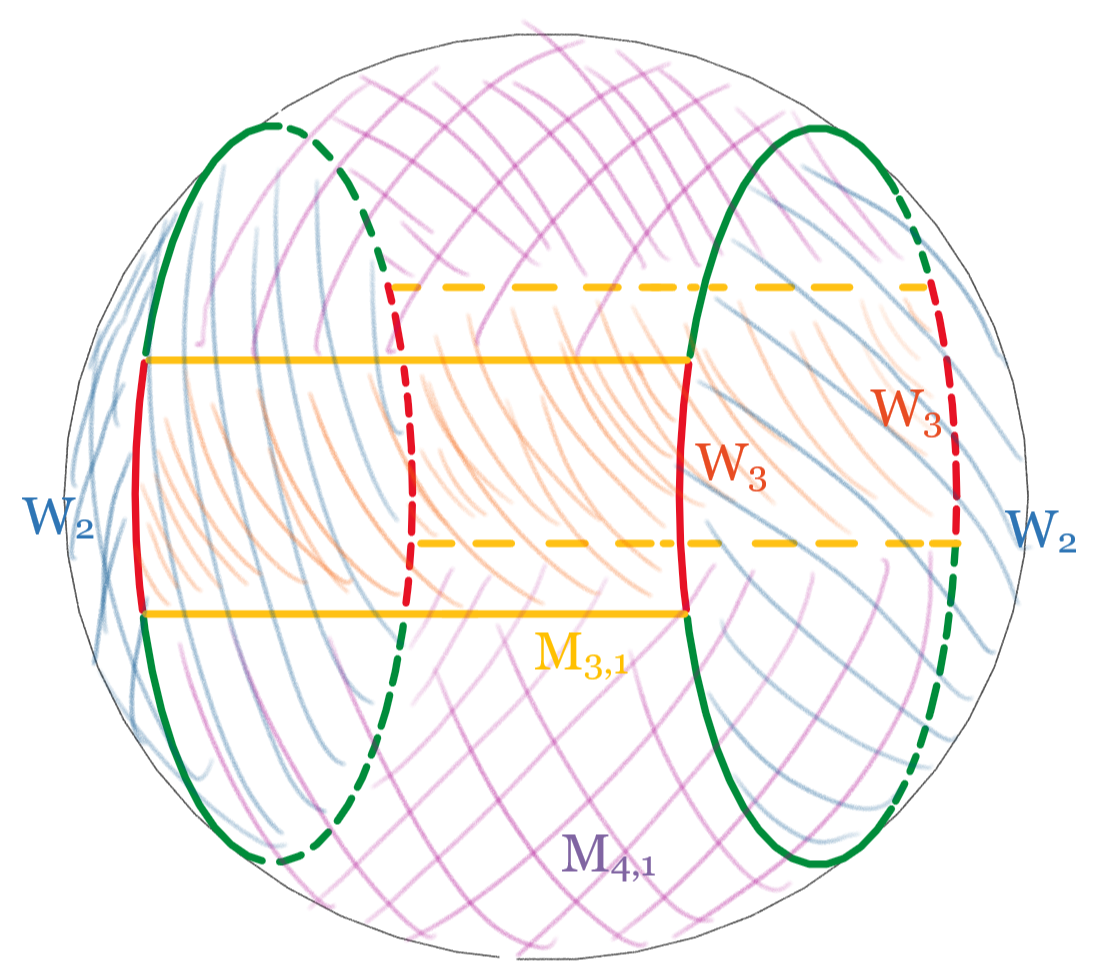
\includegraphics[width=\linewidth]{fig/Toda Manifold drawing - with M labels.png}
  \captionof{figure}{
  We can see that $\colim D_{*}$ is a topological space that inherits a closed smooth manifold structure.
  }
  \label{fig:differential}
\end{minipage}
\end{figure}

\newpage
\begin{restatable}{thmA}{ThA}\label{SSofStrFFCat}
    Let $\fC$ be a flow category with an $\cX$-tangential structure. There is a spectral sequence:
    \begin{equation*}
        \pg{E}{1}{n}{p} = \bigoplus_{\norm{z}=p} \Omega^{\cX}_{n-p}
    \end{equation*}
    which converges to the homotopy groups of the realization:
    \begin{equation*}
        \rnp{E} \implies \pi_n \norm{\fC}.
    \end{equation*}
    An element $W_p=\{W_z\} \in \pg{E}{1}{n}{p}$ survives to $\pg{E}{r+1}{n}{p}$ if and only if we can extend the collection $W_p$ to an right flow module, over $\fC_{[p,p-r]}$. The differential is represented geometrically by the Toda manifolds:
    \begin{equation*}
        d_{r+1}(W_p) = \{\flowM_{-,z} \circ W\}_{z \in \fC_{p-(r+1)}} \in \bigoplus_{z \in \fC_{p-(r+1)}} \Omega^{\cX}_{n-p+r} = \pg{E}{r+1}{n-1}{p-(r+1)}
    \end{equation*}\todo{write as $\bigcup$}
\end{restatable}

A key tool used to prove \cref{SSofStrFFCat} is a description of the spectral sequence associated with a coherent chain complex expressed in terms of chain complex maps.

\begin{restatable}{thmA}{ThB}\label{SSofCh}
    Let $K \in \Ch(\Sp)$ be a coherent chain complex in Spectra. Then there is a spectral sequence:
    \begin{equation*}
        E_1^{n,p} = \pi_{n - p} K_p,
    \end{equation*}
    which converges to
    \begin{equation*}
        E_r^{n,p} \implies \pi_n \colim_p (\cI K)_p,
    \end{equation*}
    
    Moreover, let $x: \mathbb{S}^{n - p} \to K_p$ represent an element of $\pg{E}{1}{n}{p}$. Then $x$ survives to $\pg{E}{r+1}{n}{p}$ if and only if there exists a chain map:
    \begin{equation}\label{eq:x_ext}
        \xymatrix{
        \mathbb{S}^{n - p} \ar[d]_{x} \ar[r] & 0 \ar[r]\ar[d] & \dots \ar[r]\ar[d]& 0\ar[d]\\
        K_p \ar[r]^{d_p}& K_{p - 1} \ar[r]^{d_{p - 1}}& \dots \ar[r]^{d_{p - r} \quad}& K_{p - r}
        }
    \end{equation}
    Here, the top row is concentrated in degree $p$, and the bottom row is the restriction of $K$ from degree $p$ down to $p-r$.
    The differential $\partial_{r+1}(x)$ is given by the composition of chain maps:
    \begin{equation*}
        \xymatrix
        {   \mathbb{S}^{n-p} \ar[r]\ar[d]_x & \dots \ar[r]\ar[d] &  0 \ar[d]\\
            K_p \ar[r]\ar[d] & \dots \ar[r]\ar[d] &  K_{p-r} \ar[d] \\
            0 \ar[r] & \dots \ar[r] & K_{p-r-1} 
        }
    \end{equation*}
    The first map is precisely \cref{eq:x_ext} and the second is induced by the structure of the chain complex $K$.
\end{restatable}
We obtain this result by combining the description of the spectral sequence of a filtered object in Lurie \cite{Lur17} with the results of~\cite{Ari21}.

\subsection*{Relation to other work}\todo{Delete everything which is not directly related to flow categories (delete all the Khovanov, Arnold, knots,...)}
This paper contributes to the broader project of providing a geometric model for spectra. For the foundation of this project, which defines the stable $\infty$-category of framed flow categories and establishes its equivalence with the category of spectra, see \cite{abouzaid2024foundation}.

This project traces back to the work of Cohen-Jones-Segal (CJS) in \cite{CJS95}, where the term “flow category” was introduced as a means of organizing the data of a Morse-Smale function in a categorical way. In that work, a coherent version of chain complexes is constructed from such a category, and these chains are subsequently “realized” as a filtered spectrum. These ideas have since proven very useful in Floer theory.

In knot theory, organizing the data of knots into a flow category results in a stable homotopy type that lifts Khovanov homology (see \cite{LS14}). Moreover, by simplifying the flow categories (see \cite{lobb2018framed, lobb2017calculus}) and classifying $0$- and $1$-dimensional manifolds, one obtains a combinatorial description and an effective algorithm for computing the operations
\[
    \operatorname{Sq}^2 : H^\ast(\fC, \mathbb{Z}/2) \to H^{\ast+2}(\fC, \mathbb{Z}/2)
\]
from a knot diagram. This leads to the calculation of the corresponding homotopy (see \cite{lobb2020khovanov, lipshitz2014steenrod}). For a recap of flow categories in Khovanov and knot Floer theories, see \cite{marengon2024spectra}.

Our work is similar in spirit to these developments in that we use higher flow manifolds to compute the differentials, which can be interpreted as higher cohomology operations.

In Hamiltonian Floer theory, one of the breakthroughs related to the Arnold conjecture employed a CJS-like construction—a generalization of flow categories adapted to Hamiltonian flow data—to prove a version of the Arnold conjecture over a field of characteristic $p$ (see \cite{abouzaid2021arnold}). Similar ideas appear in the work on the integral Arnold conjecture (see \cite{rezchikov2022integral, bai2022arnold}). Another recent development is the theory of Morse-Bott flow categories, where the function has critical sets (rather than isolated points) (see \cite{bonciocat2024revisiting}). An ongoing line of research is the introduction of an equivariant structure on such categories, which in turn induces an equivariant structure on the realization spectrum—a framework that supports cyclotomic methods in symplectic geometry (see \cite{cote2023equivariant, rezchikov2024cyclotomic}).

One also finds flow-category-like constructions in Lagrangian geometry that lift the Fukaya category of a symplectic manifold (see \cite{porcelli2024bordism, porcelli2024spectral}).

\begin{rem}
    In this paper we treat flow categories as chain complexes in $\Sp$ or, equivalently, as filtered spectra. We expect that there is a construction analogous to that in \cite{abouzaid2024foundation} which provides a flow-categorical model for $\{K_p\} \in \Ch(\Sp)$ such that $K_p = \bigoplus \mathbb{S}$.
\end{rem}

The interpretation of gluing manifolds as Toda brackets or Massey products appears in \cite{alexander1972cobordism}, where the Massey product is defined via the gluing of two manifolds with boundary.

\Cref{SSofCh} bears a similar flavor to other works on spectral sequences associated with various objects. In \cite{Ari21}, the authors explain the connection between filtered objects and coherent chain complexes, and they also define a spectral sequence for coherent chain complexes using the Beilinson $t$-structure. We also recommend \cite{antieau2024spectral} as an introduction to spectral sequences and their relation both to chain complexes and to the spectral sequence of filtered objects defined in \cite{Lur17}. The construction of the spectral sequence in this paper is similar to that in \cite{blanc2022spectral}, where the authors define a spectral sequence associated with a simplicial object.

\subsection*{Paper layout}
Section~2 is devoted to the framework of chain complexes in (stable) $\infty$-categories and contains the proof of \Cref{SSofCh}.

In Section~3, we recall the definitions of manifolds with corners, framed flow categories, and the Pontryagin-Thom construction for manifolds with corners. At the end of this section, we demonstrate several properties of the Pontryagin-Thom construction that will be useful in later sections.

Section~4 establishes a correspondence between chain complexes in the category of spectra (with values $\bigoplus \mathbb{S}$) and framed flow categories.

Our goal in Sections~5 and~6 is to upgrade this correspondence so that it interacts naturally with spectral sequences. In other words, given a framed flow category, we show how to produce a spectral sequence for the corresponding chain complex and provide a geometrical description of its pages and differentials.

In Section~5, we compare various models for chain complexes by considering different models for $\infty$-categories (namely, topologically enriched, simplicially enriched, and simplicial sets). This comparison allows us to give a straightforward description of the composition of maps between flow categories.

Section~6 translates this description of composition into a geometrical framework and establishes the existence of a spectral sequence associated with framed flow categories.

In the final section, we explain how the framing structure can be replaced by a more general tangential structure, and we discuss how different structures interact. This section also contains examples of spectral sequences arising from flow categories.

\subsection*{Discussion and open problems}
\textbf{Different definitions for flow categories.} In \cite{abouzaid2024foundation}, the authors construct an $\infty$-category $\mathrm{Flow}^{\fr}$ (see also \cite{porcelli2024bordism} for the homotopy category) and show that it is equivalent to $\Sp$. We now explain the main difference between their work and ours from an algebro-topological perspective. Let $M$ be a compact manifold. Given two Morse-Smale functions $f$ and $g$, one obtains two framed flow categories, $\fC_f$ and $\fC_g$. By interpolating between $f$ and $g$, we obtain two maps in $\mathrm{Flow}^{\fr}$
\[
    H_{f,g}: \fC_f \to \fC_g, \quad H_{g,f}: \fC_g \to \fC_f,
\]
and by homotoping the compositions we obtain 2-morphisms
\[
    H_{g,f} \circ H_{f,g} \simeq \mathrm{Id}, \quad H_{f,g} \circ H_{g,f} \simeq \mathrm{Id}.
\]
Hence, the flow category of $M$ is independent of the choice of Morse-Smale function.

On the other hand, the functions $f$ and $g$ induce CW structures on $M$, and different CW structures yield different (Atiyah-Hirzebruch) spectral sequences. Therefore, one cannot define a spectral sequence as an invariant of the equivalence classes in $\mathrm{Flow}^{\fr}$.

To address this issue, we conjecture that one can define another $\infty$-category, with a modified class of morphisms. Specifically, for a 2-morphism $R$ between flow categories $\fC$ and $\sD$, and for objects $x \in \fC$ and $y \in \sD$, we require that if $\|y\| > \|x\|$, then $R_{x,y} = \varnothing$ (rather than being a manifold of dimension $\|y\| - \|x\|$). This construction should yield a subcategory of $\Fil(\Sp)$ in which the two Morse-Smale functions on a manifold $M$ produce distinct objects.

Using this perspective, we can think of \cref{SSofStrFFCat} as a spectral sequence of filtered flow category $F \in \Fil(\mathrm{Flow}^{\cX})$ where the filtration is induces by the index filtration on a flow category.

In this paper the full $\infty$-categorical structure is unnecessary; instead, we define the equivalence relation on flow categories by pulling it back from the category $\Ch(\Sp)$ (see \Cref{prop:FF_are_Ch}).